\documentclass[final,3p,times]{elsarticle}

\usepackage[T1]{fontenc}
\usepackage[utf8]{inputenc}
\usepackage{amsmath,amssymb}
\usepackage{booktabs}
\usepackage{array}
\usepackage{graphicx}
\usepackage{microtype}
\usepackage{xurl}
\usepackage{algorithm}
\usepackage{algpseudocode}
\usepackage{placeins}
\usepackage[hidelinks]{hyperref}

\makeatletter
\let\ps@pprintTitle\ps@plain
\makeatother

\graphicspath{{figures/}}
\hyphenation{Dilated-RNN}

% Float placement: let floats share pages with running text instead of
% forming dedicated float pages that leave the rest of the page blank.
\renewcommand{\topfraction}{0.9}
\renewcommand{\bottomfraction}{0.7}
\renewcommand{\textfraction}{0.07}
\renewcommand{\floatpagefraction}{0.85}
\renewcommand{\dbltopfraction}{0.9}
\renewcommand{\dblfloatpagefraction}{0.85}
\setcounter{topnumber}{3}
\setcounter{bottomnumber}{2}
\setcounter{totalnumber}{4}
\setcounter{dbltopnumber}{3}
\renewcommand{\thetable}{S\arabic{table}}
\renewcommand{\thefigure}{S\arabic{figure}}
\begin{document}
\raggedbottom

\begin{frontmatter}
\title{Supplementary Material for\\
``Multi-Resolution Solar Irradiance Forecasting:\\
A Comparative Study of TimesNet and DilatedRNN''}
\author[unicamp]{Gustavo de Melo Nascimento}
\author[unicamp]{Thales Wulfert Cabral}
\author[unicamp]{Gustavo Fraidenraich}
\address[unicamp]{School of Electrical and Computer Engineering,
University of Campinas, Campinas, SP, Brazil}
\end{frontmatter}

\section{Complete Reference-Model Benchmark}
This supplement compares TimesNet and DilatedRNN with all evaluated reference
models at each cumulative forecast horizon.
Tables~\ref{tab:baseline_hourly_72_extension_24}--\ref{tab:baseline_monthly_6_6}
report MAE, MSE, RMSE, nRMSE, and $R^2$ for every task and checkpoint.
Figure~\ref{fig:supp_ranking} summarizes the resulting macro-MAE ranks, and
Figure~\ref{fig:supp_seeds} summarizes variability across random seeds for
the seven stochastic learned models.
\begin{table}[!htbp]
\centering
\small
\setlength{\tabcolsep}{6pt}
\caption{Hourly: cumulative scores through 24 h. MAE and RMSE are in W/m$^2$, MSE in (W/m$^2$)$^2$, nRMSE in percent, and $R^2$ is dimensionless. Bold/underline indicate best/second-best values before rounding.}
\label{tab:baseline_hourly_72_extension_24}
\begin{tabular}{@{}lrrrrr@{}}
\toprule
Model & MAE & MSE & RMSE & nRMSE (\%) & $R^2$ \\
\midrule
Persistence & 52.58 & 15422.87 & 122.21 & 61.28 & 0.801 \\
Seasonal na\"ive & 65.91 & 20925.50 & 142.78 & 71.19 & 0.734 \\
ARIMA & 129.76 & 51450.37 & 225.60 & 109.24 & 0.396 \\
XGBoost & \textbf{48.37} & \textbf{9481.34} & \textbf{96.05} & \textbf{47.95} & \textbf{0.879} \\
GRU & 49.97 & \underline{9715.60} & \underline{97.24} & \underline{48.57} & 0.876 \\
LSTM & 50.91 & 10253.35 & 100.01 & 49.95 & 0.869 \\
Transformer & 51.30 & 10394.27 & 100.84 & 50.22 & 0.868 \\
Informer & 142.27 & 64887.96 & 253.61 & 122.47 & 0.242 \\
DilatedRNN & 50.73 & 10481.55 & 101.18 & 50.49 & 0.867 \\
TimesNet & \underline{49.39} & 9722.15 & 97.29 & 48.57 & \underline{0.876} \\
\bottomrule
\end{tabular}
\end{table}

\begin{table}[!htbp]
\centering
\small
\setlength{\tabcolsep}{6pt}
\caption{Hourly: cumulative scores through 48 h. MAE and RMSE are in W/m$^2$, MSE in (W/m$^2$)$^2$, nRMSE in percent, and $R^2$ is dimensionless. Bold/underline indicate best/second-best values before rounding.}
\label{tab:baseline_hourly_72_extension_48}
\begin{tabular}{@{}lrrrrr@{}}
\toprule
Model & MAE & MSE & RMSE & nRMSE (\%) & $R^2$ \\
\midrule
Persistence & 56.16 & 17019.73 & 128.35 & 64.34 & 0.781 \\
Seasonal na\"ive & 65.92 & 20930.30 & 142.79 & 71.21 & 0.734 \\
ARIMA & 133.57 & 55286.88 & 234.08 & 113.30 & 0.351 \\
XGBoost & \textbf{49.81} & \textbf{9914.22} & \textbf{98.23} & \textbf{49.02} & \textbf{0.874} \\
GRU & \underline{50.97} & \underline{10155.51} & \underline{99.44} & \underline{49.62} & \underline{0.871} \\
LSTM & 52.79 & 10860.92 & 103.00 & 51.39 & 0.862 \\
Transformer & 52.84 & 10874.75 & 103.12 & 51.35 & 0.862 \\
Informer & 134.21 & 57973.96 & 239.57 & 115.74 & 0.323 \\
DilatedRNN & 52.15 & 11006.84 & 103.71 & 51.73 & 0.860 \\
TimesNet & 52.16 & 10336.02 & 100.41 & 50.06 & 0.869 \\
\bottomrule
\end{tabular}
\end{table}

\begin{table}[!htbp]
\centering
\small
\setlength{\tabcolsep}{6pt}
\caption{Hourly: cumulative scores through 72 h. MAE and RMSE are in W/m$^2$, MSE in (W/m$^2$)$^2$, nRMSE in percent, and $R^2$ is dimensionless. Bold/underline indicate best/second-best values before rounding.}
\label{tab:baseline_hourly_72_extension_72}
\begin{tabular}{@{}lrrrrr@{}}
\toprule
Model & MAE & MSE & RMSE & nRMSE (\%) & $R^2$ \\
\midrule
Persistence & 58.11 & 17808.91 & 131.32 & 65.77 & 0.771 \\
Seasonal na\"ive & 65.90 & 20923.05 & 142.76 & 71.20 & 0.734 \\
ARIMA & 134.65 & 56476.00 & 236.68 & 114.51 & 0.338 \\
XGBoost & \textbf{50.50} & \textbf{10111.00} & \textbf{99.22} & \textbf{49.48} & \textbf{0.872} \\
GRU & \underline{51.52} & \underline{10354.92} & \underline{100.43} & \underline{50.08} & \underline{0.869} \\
LSTM & 53.39 & 11203.35 & 104.68 & 52.17 & 0.858 \\
Transformer & 53.22 & 11012.45 & 103.73 & 51.65 & 0.861 \\
Informer & 137.72 & 60955.61 & 245.61 & 118.55 & 0.290 \\
DilatedRNN & 52.96 & 11258.14 & 104.93 & 52.31 & 0.857 \\
TimesNet & 52.48 & 10491.15 & 101.17 & 50.41 & 0.867 \\
\bottomrule
\end{tabular}
\end{table}

\begin{table}[!htbp]
\centering
\small
\setlength{\tabcolsep}{6pt}
\caption{Daily: cumulative scores through 1 d. MAE and RMSE are in W/m$^2$, MSE in (W/m$^2$)$^2$, nRMSE in percent, and $R^2$ is dimensionless. Bold/underline indicate best/second-best values before rounding.}
\label{tab:baseline_daily_30_1}
\begin{tabular}{@{}lrrrrr@{}}
\toprule
Model & MAE & MSE & RMSE & nRMSE (\%) & $R^2$ \\
\midrule
Persistence & 43.87 & 4146.03 & 62.88 & 30.59 & 0.415 \\
Seasonal na\"ive & 58.90 & 6292.86 & 78.11 & 37.73 & 0.085 \\
Climatology & 45.74 & 3572.29 & 58.86 & 28.38 & 0.476 \\
ARIMA & \textbf{39.95} & 2886.75 & 52.77 & 25.56 & \textbf{0.586} \\
XGBoost & 41.58 & \underline{2865.16} & \underline{52.63} & \underline{25.42} & 0.581 \\
GRU & \underline{41.43} & \textbf{2851.72} & \textbf{52.54} & \textbf{25.37} & \underline{0.583} \\
LSTM & 42.04 & 2957.11 & 53.56 & 25.84 & 0.567 \\
Transformer & 44.74 & 3201.27 & 55.68 & 26.85 & 0.526 \\
Informer & 47.32 & 3584.79 & 59.07 & 28.49 & 0.480 \\
DilatedRNN & 43.27 & 2995.25 & 53.88 & 25.99 & 0.559 \\
TimesNet & 43.20 & 3057.17 & 54.42 & 26.23 & 0.547 \\
\bottomrule
\end{tabular}
\end{table}

\begin{table}[!htbp]
\centering
\small
\setlength{\tabcolsep}{6pt}
\caption{Daily: cumulative scores through 3 d. MAE and RMSE are in W/m$^2$, MSE in (W/m$^2$)$^2$, nRMSE in percent, and $R^2$ is dimensionless. Bold/underline indicate best/second-best values before rounding.}
\label{tab:baseline_daily_30_3}
\begin{tabular}{@{}lrrrrr@{}}
\toprule
Model & MAE & MSE & RMSE & nRMSE (\%) & $R^2$ \\
\midrule
Persistence & 50.17 & 5151.75 & 70.28 & 34.09 & 0.261 \\
Seasonal na\"ive & 58.98 & 6305.46 & 78.18 & 37.75 & 0.081 \\
Climatology & 45.76 & 3572.96 & 58.86 & 28.38 & 0.475 \\
ARIMA & \textbf{43.04} & 3207.32 & 55.78 & 26.93 & 0.534 \\
XGBoost & \underline{43.09} & \textbf{3026.54} & \textbf{54.14} & \textbf{26.12} & \textbf{0.554} \\
GRU & 43.41 & \underline{3030.26} & \underline{54.22} & \underline{26.13} & \underline{0.552} \\
LSTM & 43.14 & 3081.28 & 54.71 & 26.36 & 0.546 \\
Transformer & 44.69 & 3202.67 & 55.69 & 26.84 & 0.525 \\
Informer & 47.26 & 3568.12 & 58.93 & 28.41 & 0.479 \\
DilatedRNN & 43.80 & 3067.61 & 54.54 & 26.29 & 0.546 \\
TimesNet & 43.63 & 3104.70 & 54.85 & 26.42 & 0.538 \\
\bottomrule
\end{tabular}
\end{table}

\begin{table}[!htbp]
\centering
\small
\setlength{\tabcolsep}{6pt}
\caption{Daily: cumulative scores through 7 d. MAE and RMSE are in W/m$^2$, MSE in (W/m$^2$)$^2$, nRMSE in percent, and $R^2$ is dimensionless. Bold/underline indicate best/second-best values before rounding.}
\label{tab:baseline_daily_30_7}
\begin{tabular}{@{}lrrrrr@{}}
\toprule
Model & MAE & MSE & RMSE & nRMSE (\%) & $R^2$ \\
\midrule
Persistence & 53.77 & 5624.21 & 73.83 & 35.63 & 0.176 \\
Seasonal na\"ive & 59.00 & 6312.12 & 78.22 & 37.75 & 0.078 \\
Climatology & 45.75 & 3571.05 & 58.85 & 28.36 & 0.475 \\
ARIMA & 44.96 & 3400.18 & 57.56 & 27.72 & 0.502 \\
XGBoost & \underline{43.71} & \textbf{3080.29} & \textbf{54.66} & \textbf{26.33} & \textbf{0.544} \\
GRU & 44.12 & \underline{3095.66} & \underline{54.83} & \underline{26.39} & 0.539 \\
LSTM & \textbf{43.69} & 3138.82 & 55.25 & 26.59 & 0.536 \\
Transformer & 44.63 & 3208.24 & 55.72 & 26.85 & 0.523 \\
Informer & 46.86 & 3495.48 & 58.29 & 28.09 & 0.487 \\
DilatedRNN & 44.08 & 3102.68 & 54.87 & 26.42 & \underline{0.540} \\
TimesNet & 43.95 & 3137.67 & 55.14 & 26.54 & 0.531 \\
\bottomrule
\end{tabular}
\end{table}

\begin{table}[!htbp]
\centering
\small
\setlength{\tabcolsep}{6pt}
\caption{Daily: cumulative scores through 14 d. MAE and RMSE are in W/m$^2$, MSE in (W/m$^2$)$^2$, nRMSE in percent, and $R^2$ is dimensionless. Bold/underline indicate best/second-best values before rounding.}
\label{tab:baseline_daily_30_14}
\begin{tabular}{@{}lrrrrr@{}}
\toprule
Model & MAE & MSE & RMSE & nRMSE (\%) & $R^2$ \\
\midrule
Persistence & 56.41 & 5976.80 & 76.16 & 36.69 & 0.120 \\
Seasonal na\"ive & 58.91 & 6303.03 & 78.15 & 37.69 & 0.078 \\
Climatology & 45.64 & 3559.89 & 58.74 & 28.29 & 0.476 \\
ARIMA & 46.79 & 3620.05 & 59.44 & 28.59 & 0.472 \\
XGBoost & \textbf{43.96} & \textbf{3105.04} & \textbf{54.86} & \textbf{26.41} & \textbf{0.539} \\
GRU & 44.42 & 3122.00 & 55.05 & 26.47 & 0.534 \\
LSTM & \underline{44.00} & 3169.16 & 55.51 & 26.69 & 0.531 \\
Transformer & 44.38 & 3182.43 & 55.48 & 26.71 & 0.525 \\
Informer & 46.17 & 3389.47 & 57.33 & 27.61 & 0.499 \\
DilatedRNN & 44.11 & \underline{3114.01} & \underline{54.94} & \underline{26.44} & \underline{0.537} \\
TimesNet & 44.09 & 3150.30 & 55.23 & 26.57 & 0.529 \\
\bottomrule
\end{tabular}
\end{table}

\begin{table}[!htbp]
\centering
\small
\setlength{\tabcolsep}{6pt}
\caption{Daily: cumulative scores through 30 d. MAE and RMSE are in W/m$^2$, MSE in (W/m$^2$)$^2$, nRMSE in percent, and $R^2$ is dimensionless. Bold/underline indicate best/second-best values before rounding.}
\label{tab:baseline_daily_30_30}
\begin{tabular}{@{}lrrrrr@{}}
\toprule
Model & MAE & MSE & RMSE & nRMSE (\%) & $R^2$ \\
\midrule
Persistence & 60.28 & 6478.87 & 79.47 & 38.26 & 0.055 \\
Seasonal na\"ive & 58.78 & 6290.25 & 78.05 & 37.67 & 0.081 \\
Climatology & 45.51 & 3545.97 & 58.61 & 28.25 & 0.480 \\
ARIMA & 50.69 & 4109.72 & 63.52 & 30.52 & 0.411 \\
XGBoost & 43.93 & \textbf{3094.87} & \textbf{54.76} & \textbf{26.37} & \textbf{0.542} \\
GRU & 44.23 & 3112.23 & 54.95 & 26.44 & 0.537 \\
LSTM & 44.18 & 3180.94 & 55.64 & 26.76 & 0.530 \\
Transformer & \underline{43.88} & 3139.28 & 55.12 & 26.54 & 0.533 \\
Informer & 45.47 & 3316.80 & 56.75 & 27.32 & 0.510 \\
DilatedRNN & \textbf{43.85} & \underline{3097.20} & \underline{54.79} & \underline{26.38} & \underline{0.541} \\
TimesNet & 44.08 & 3143.38 & 55.16 & 26.55 & 0.531 \\
\bottomrule
\end{tabular}
\end{table}

\begin{table}[!htbp]
\centering
\small
\setlength{\tabcolsep}{6pt}
\caption{Monthly, one step: cumulative scores through 1 mo. MAE and RMSE are in W/m$^2$, MSE in (W/m$^2$)$^2$, nRMSE in percent, and $R^2$ is dimensionless. Bold/underline indicate best/second-best values before rounding.}
\label{tab:baseline_monthly_1_1}
\begin{tabular}{@{}lrrrrr@{}}
\toprule
Model & MAE & MSE & RMSE & nRMSE (\%) & $R^2$ \\
\midrule
Persistence & 35.09 & 1808.74 & 42.17 & 20.89 & 0.576 \\
Seasonal na\"ive & 16.94 & 496.86 & 21.37 & 10.38 & 0.829 \\
Climatology & \textbf{12.57} & \textbf{248.57} & \textbf{15.55} & \textbf{7.77} & \textbf{0.930} \\
ARIMA & 16.26 & 430.61 & 19.97 & 9.85 & 0.859 \\
XGBoost & 14.82 & 336.01 & 18.01 & 8.85 & 0.891 \\
GRU & 13.86 & 317.13 & 17.06 & 8.32 & 0.889 \\
LSTM & 14.27 & 327.98 & 17.44 & 8.45 & 0.886 \\
Transformer & 13.12 & 303.83 & 16.50 & 8.20 & 0.897 \\
Informer & \underline{12.85} & 281.04 & 16.20 & 8.02 & 0.907 \\
DilatedRNN & 13.01 & \underline{270.75} & \underline{16.02} & \underline{7.86} & \underline{0.909} \\
TimesNet & 13.89 & 337.10 & 17.49 & 8.51 & 0.882 \\
\bottomrule
\end{tabular}
\end{table}

\begin{table}[!htbp]
\centering
\small
\setlength{\tabcolsep}{6pt}
\caption{Monthly, six steps: cumulative scores through 1 mo. MAE and RMSE are in W/m$^2$, MSE in (W/m$^2$)$^2$, nRMSE in percent, and $R^2$ is dimensionless. Bold/underline indicate best/second-best values before rounding.}
\label{tab:baseline_monthly_6_1}
\begin{tabular}{@{}lrrrrr@{}}
\toprule
Model & MAE & MSE & RMSE & nRMSE (\%) & $R^2$ \\
\midrule
Persistence & 33.19 & 1755.43 & 41.62 & 18.96 & 0.565 \\
Seasonal na\"ive & 16.50 & 464.32 & 20.48 & 9.12 & 0.842 \\
Climatology & \textbf{13.61} & \textbf{268.51} & \textbf{16.23} & \textbf{7.48} & \textbf{0.920} \\
ARIMA & 16.13 & 433.94 & 20.21 & 9.28 & 0.853 \\
XGBoost & 14.73 & 328.11 & 17.90 & 8.18 & \underline{0.895} \\
GRU & 15.45 & 387.09 & 18.97 & 8.55 & 0.862 \\
LSTM & 15.74 & 409.49 & 19.47 & 8.73 & 0.854 \\
Transformer & 15.71 & 379.84 & 18.77 & 8.60 & 0.875 \\
Informer & \underline{14.06} & \underline{321.22} & \underline{17.29} & \underline{7.95} & 0.893 \\
DilatedRNN & 14.89 & 357.95 & 18.25 & 8.22 & 0.875 \\
TimesNet & 14.86 & 393.02 & 18.99 & 8.49 & 0.864 \\
\bottomrule
\end{tabular}
\end{table}

\begin{table}[!htbp]
\centering
\small
\setlength{\tabcolsep}{6pt}
\caption{Monthly, six steps: cumulative scores through 3 mo. MAE and RMSE are in W/m$^2$, MSE in (W/m$^2$)$^2$, nRMSE in percent, and $R^2$ is dimensionless. Bold/underline indicate best/second-best values before rounding.}
\label{tab:baseline_monthly_6_3}
\begin{tabular}{@{}lrrrrr@{}}
\toprule
Model & MAE & MSE & RMSE & nRMSE (\%) & $R^2$ \\
\midrule
Persistence & 61.45 & 5874.46 & 74.97 & 31.39 & -0.855 \\
Seasonal na\"ive & 17.06 & 487.59 & 21.05 & 8.77 & 0.778 \\
Climatology & \textbf{13.08} & \textbf{258.73} & \textbf{15.94} & \textbf{6.81} & \textbf{0.893} \\
ARIMA & 18.61 & 563.81 & 23.02 & 9.68 & 0.760 \\
XGBoost & 14.93 & 329.96 & 17.96 & 7.56 & 0.860 \\
GRU & 14.81 & 369.34 & 18.34 & 7.69 & 0.818 \\
LSTM & 15.33 & 388.44 & 18.84 & 7.88 & 0.809 \\
Transformer & 14.43 & 338.72 & 17.69 & 7.52 & 0.841 \\
Informer & \underline{13.15} & \underline{293.58} & \underline{16.54} & \underline{7.04} & \underline{0.861} \\
DilatedRNN & 14.33 & 331.88 & 17.52 & 7.36 & 0.839 \\
TimesNet & 14.49 & 364.96 & 18.32 & 7.66 & 0.829 \\
\bottomrule
\end{tabular}
\end{table}

\begin{table}[!htbp]
\centering
\small
\setlength{\tabcolsep}{6pt}
\caption{Monthly, six steps: cumulative scores through 6 mo. MAE and RMSE are in W/m$^2$, MSE in (W/m$^2$)$^2$, nRMSE in percent, and $R^2$ is dimensionless. Bold/underline indicate best/second-best values before rounding.}
\label{tab:baseline_monthly_6_6}
\begin{tabular}{@{}lrrrrr@{}}
\toprule
Model & MAE & MSE & RMSE & nRMSE (\%) & $R^2$ \\
\midrule
Persistence & 91.89 & 12746.86 & 109.59 & 46.64 & -2.489 \\
Seasonal na\"ive & 18.00 & 540.29 & 22.38 & 9.51 & 0.773 \\
Climatology & \textbf{13.03} & \textbf{266.71} & \textbf{16.10} & \textbf{6.98} & \textbf{0.901} \\
ARIMA & 19.17 & 588.67 & 23.64 & 10.01 & 0.781 \\
XGBoost & 14.72 & 322.88 & 17.76 & 7.59 & \underline{0.873} \\
GRU & 14.40 & 352.35 & 17.77 & 7.56 & 0.840 \\
LSTM & 14.76 & 360.10 & 18.11 & 7.69 & 0.838 \\
Transformer & 14.43 & 340.41 & 17.69 & 7.65 & 0.855 \\
Informer & \underline{13.88} & \underline{319.87} & \underline{17.26} & \underline{7.47} & 0.866 \\
DilatedRNN & 14.37 & 331.63 & 17.47 & 7.47 & 0.855 \\
TimesNet & 14.46 & 357.67 & 18.24 & 7.77 & 0.850 \\
\bottomrule
\end{tabular}
\end{table}

\begin{figure}[!htbp]
\centering
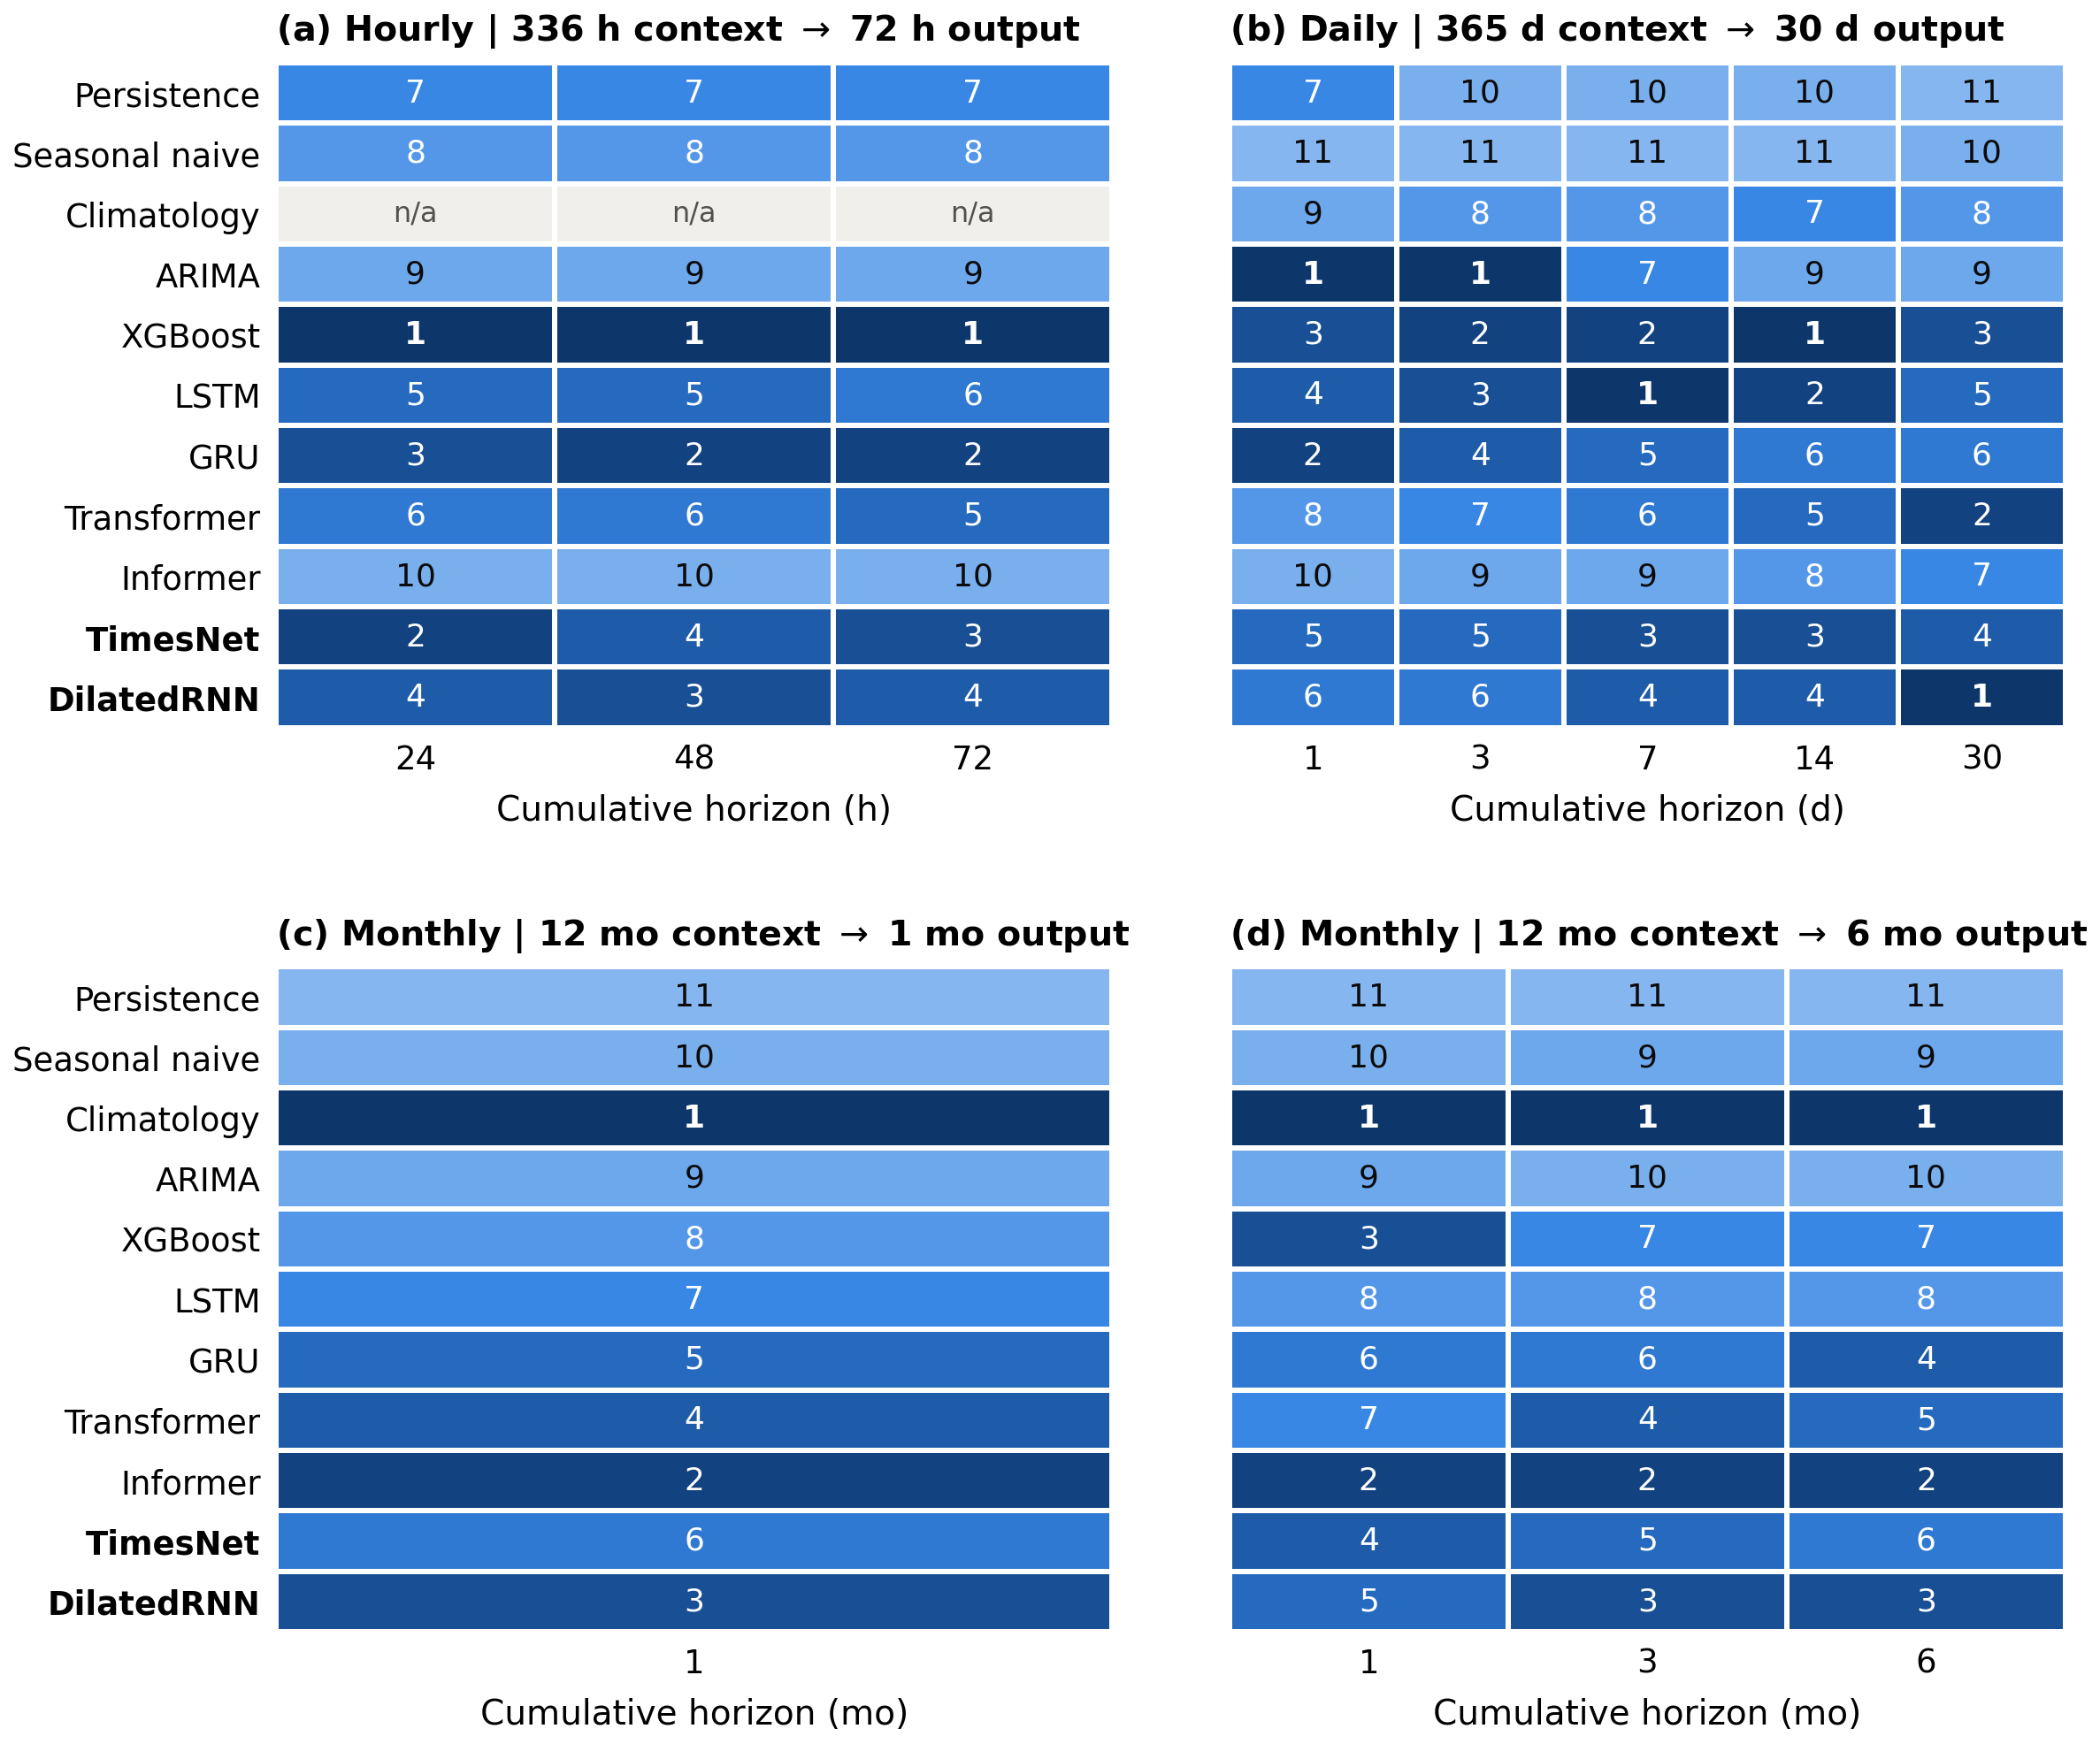
\includegraphics[width=0.90\textwidth]{ranking_por_tarefa.png}
\caption{Macro-MAE rank of each model at every cumulative forecast horizon.
Rank 1 (darkest) indicates the lowest MAE within a task and horizon; tied
models share the better rank. Hourly results use seed 42, and the other
learned models use five-seed ensembles. Hourly climatology was not
evaluated (n/a).}
\label{fig:supp_ranking}
\end{figure}
\begin{figure}[!htbp]
\centering
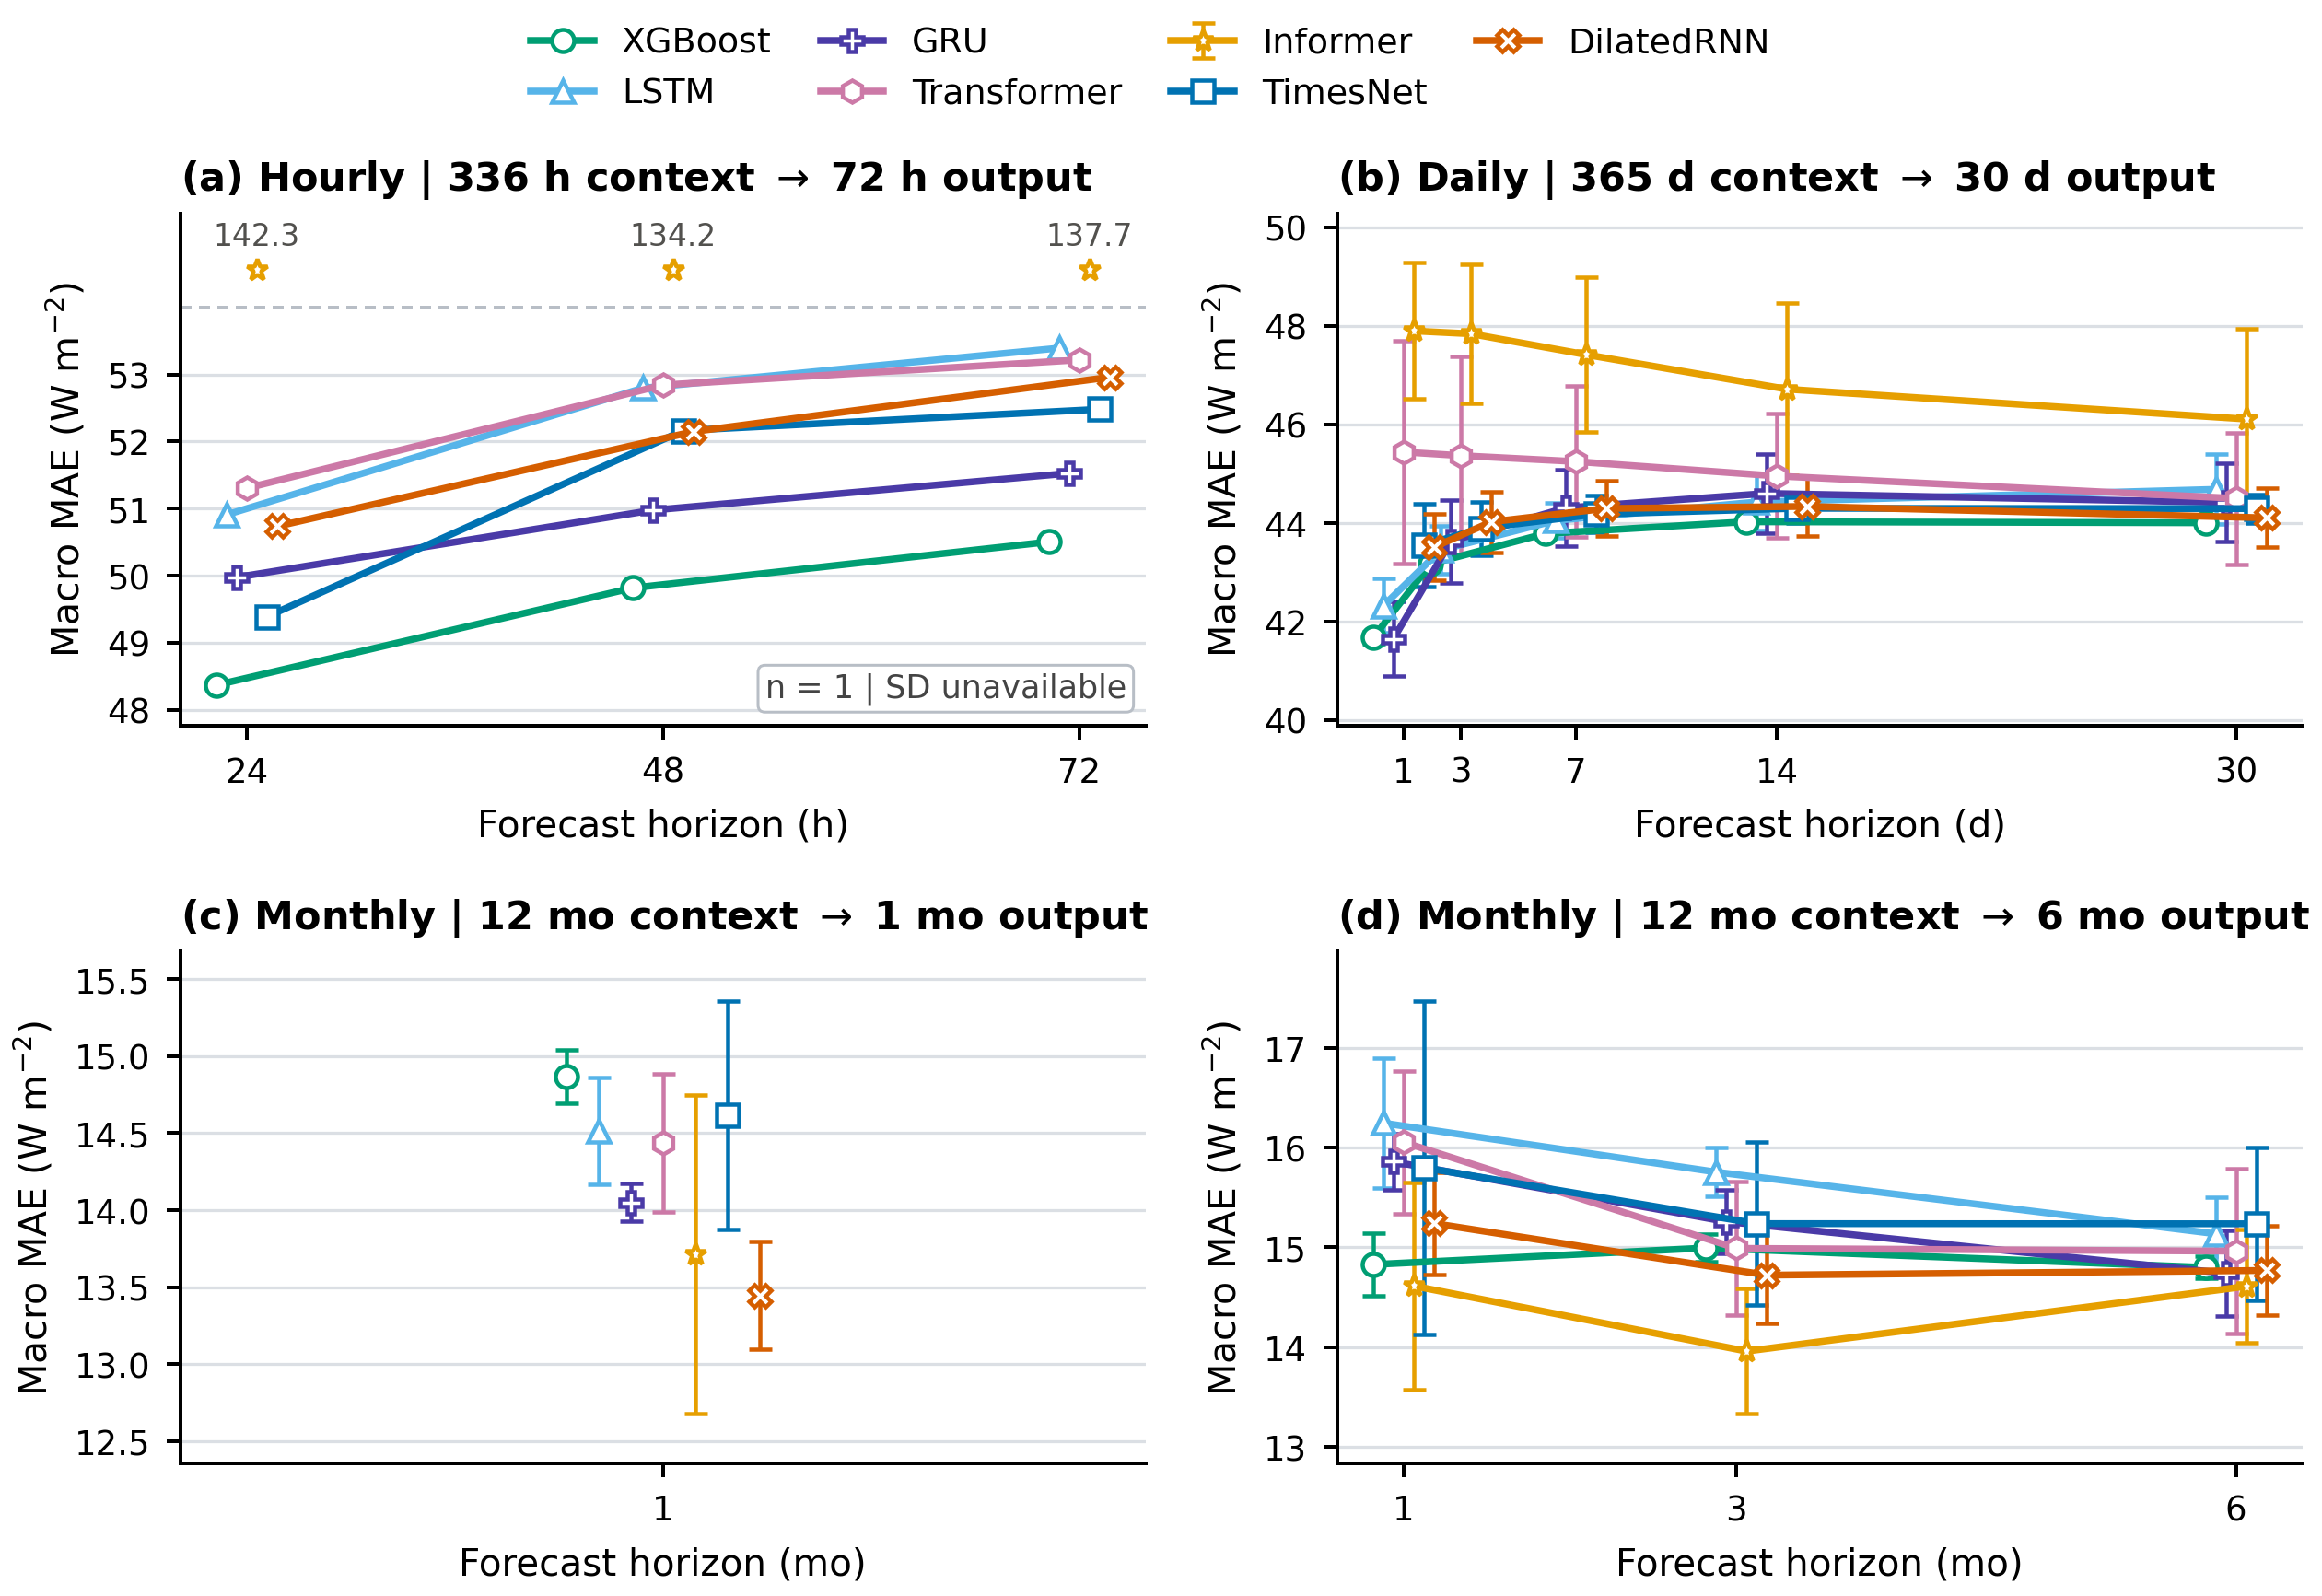
\includegraphics[width=0.90\textwidth]{variabilidade_por_semente.png}
\caption{Seed-level macro-MAE of the seven stochastic learned models: means
with error bars spanning one sample standard deviation. Markers are offset
horizontally for legibility. Hourly runs use seed 42 only and have no error
bars; the hourly Informer lies above the plotted range, so its markers sit
above the dashed line with their values printed.}
\label{fig:supp_seeds}
\end{figure}
\FloatBarrier
\section{Detailed Forecasting Algorithms}

The three blocks below provide additional preparation and evaluation details
for the protocol and architecture pseudocode in the main article. They focus
on the matched TimesNet--DilatedRNN comparison.
Algorithm~\ref{alg:supp-block-a} defines data preparation,
Algorithm~\ref{alg:supp-block-b} specifies selection and refitting, and
Algorithm~\ref{alg:supp-block-c} records post-processing and evaluation.

\setcounter{algorithm}{0}
\renewcommand{\thealgorithm}{S\arabic{algorithm}}

\begin{algorithm}[H]
\caption{Leakage-controlled data preparation}
\label{alg:supp-block-a}
\footnotesize
\begin{algorithmic}[1]
\Require Site series $\{y_{\ell,t}\}$; task $(r,C,H)$; fixed cuts
\Ensure Aligned fit, validation, refit, and test windows
\For{each site $\ell$}
  \State parse, sort, and verify a complete nonnegative GHI series
  \If{$r$ is monthly}
    \State aggregate daily GHI by civil-month arithmetic mean
  \EndIf
  \State assign the fixed identifier $\ell$
  \State fit $s_{\ell}^{\mathrm{sel}}$ using observations before 2023
  \State fit $s_{\ell}^{\mathrm{refit}}$ using observations before 2024
  \For{each declared partition $P$}
    \State form contexts $y_{\ell,t-C:t-1}$ with site ID $\ell$
    \State retain only full targets $y_{\ell,t:t+H-1}$ lying in $P$
    \State assert the expected origin count and chronological boundaries
  \EndFor
\EndFor
\State concatenate sites and sort each partition by origin and site identifier
\end{algorithmic}
\end{algorithm}

\begin{algorithm}[H]
\caption{TimesNet--DilatedRNN selection and direct forecasting}
\label{alg:supp-block-b}
\footnotesize
\begin{algorithmic}[1]
\Require Block-A partitions; frozen seeds and model settings
\Ensure Validation and test forecasts on common origins in W/m$^2$
\If{hourly extension}
  \State verify hashes and load the official TimesNet seed-42 forecasts
  \State $\mathcal M\gets\{\mathrm{DilatedRNN}\}$; $\mathcal S\gets\{42\}$
\Else
  \State $\mathcal M\gets\{\mathrm{TimesNet,DilatedRNN}\}$
  \State $\mathcal S\gets\{11,23,42,67,89\}$
\EndIf
\State scale fit/validation with $s_{\ell}^{\mathrm{sel}}$ and refit/test with $s_{\ell}^{\mathrm{refit}}$
\For{each $(m,s)\in\mathcal M\times\mathcal S$}
  \State initialize $m$ with seed $s$ and fit the adjustment partition using Adam
  \State select $E^\star$ by 2023 normalized MSE and early stopping
  \State retain the validation forecast from the $E^\star$ checkpoint
  \State reinitialize $m$ with seed $s$
  \State refit on the pre-2024 partition for exactly $E^\star$ epochs
  \State forecast all $H$ targets at every 2024 origin with fixed weights
  \State invert $s_{\ell}^{\mathrm{sel}}$ for validation and $s_{\ell}^{\mathrm{refit}}$ for test
  \State retain both unbounded seed forecasts in W/m$^2$
\EndFor
\State for daily/monthly models, average the five raw seed forecasts
\State retain seed and ensemble forecasts separately, before the zero floor
\end{algorithmic}
\end{algorithm}

\begin{algorithm}[H]
\caption{Post-processing, metrics, and contextual analysis}
\label{alg:supp-block-c}
\footnotesize
\begin{algorithmic}[1]
\Require Block-B forecasts; targets; declared horizons; context metadata
\Ensure Site-level, macro, horizon-wise, and contextual evidence
\For{each newly computed seed or ensemble forecast}
  \State apply $\widehat y\leftarrow\max(\widehat y,0)$ in W/m$^2$
  \If{the task is hourly}
    \State compute solar elevation at each hourly interval's midpoint
    \State set $\widehat y=0$ wherever solar elevation is nonpositive
  \EndIf
\EndFor
\State verify common site, origin, target timestamp, and lead keys
\For{each site and declared horizon}
  \State compute metrics for the cumulative prefix and the exact lead
\EndFor
\State average site metrics with equal site weight
\State form TimesNet--DilatedRNN differences paired by site
\State attach climate and adverse-day labels only after errors are fixed
\end{algorithmic}
\end{algorithm}


\section{Supporting Design and Literature Tables}
Table~\ref{tab:study_design} summarizes the four forecasting tasks and their
origin counts. Tables~\ref{tab:literature_review_short},
\ref{tab:literature_review_multistep}, and \ref{tab:literature_review_long}
cover three groups of studies, respectively: intra-hour and short hourly
forecasting; day-ahead and direct multi-step forecasting; and monthly,
multi-climate, and very-long-horizon forecasting.
\begin{table*}[!t]
\centering
\caption{Fixed multi-resolution forecasting tasks.}
\label{tab:study_design}
\footnotesize
\setlength{\tabcolsep}{2.3pt}
\renewcommand{\arraystretch}{1.12}
\begin{tabular}{@{}
  >{\raggedright\arraybackslash}p{0.16\linewidth}
  >{\centering\arraybackslash}p{0.18\linewidth}
  >{\centering\arraybackslash}p{0.19\linewidth}
  >{\centering\arraybackslash}p{0.22\linewidth}
  >{\raggedright\arraybackslash}p{0.17\linewidth}@{}}
\toprule
\textbf{Task} & \textbf{Context $\to$ output} &
\textbf{Evaluated horizons} & \textbf{Origins/site A/V/R/T} &
\textbf{Role} \\
\midrule
Hourly & 336 h $\to$ 72 h & 24, 48, 72 h &
1,445/363/1,810/363 & Official protocol; DilatedRNN seed-42 extension \\
Daily & 365 d $\to$ 30 d & 1, 3, 7, 14, 30 d &
1,067/336/1,432/337 & Primary matched task \\
Monthly-1 & 12 mo $\to$ 1 mo & 1 mo &
36/12/48/12 & Primary monthly task \\
Monthly-6 & 12 mo $\to$ 6 mo & 1, 3, 6 mo &
31/7/43/7 & Exploratory multi-month task \\
\bottomrule
\end{tabular}

\medskip
\parbox{\linewidth}{\scriptsize
A/V/R/T denote initial training (adjustment), 2023 validation, pre-2024 refit,
and 2024 test.
Every count is the number of complete forecast origins per site. Reported
multi-step horizons are evaluated both as cumulative prefixes and exact leads.}
\end{table*}

\begin{table}[!htbp]
\centering
\caption{Representative forecasting studies at intra-hour and short
hourly horizons. The studies use different targets and test protocols, so
their results are not directly ranked.}
\label{tab:literature_review}
\label{tab:literature_review_short}
\scriptsize
\setlength{\tabcolsep}{2.5pt}
\renewcommand{\arraystretch}{1.12}
\begin{tabular}{@{}p{0.11\linewidth}p{0.18\linewidth}p{0.22\linewidth}p{0.18\linewidth}p{0.25\linewidth}@{}}
\toprule
\textbf{Study} & \textbf{Target and scope} & \textbf{Inputs and processing} &
\textbf{Predictor} & \textbf{Horizon and evaluation design} \\
\midrule
Chow et al.\ \cite{chow2011} &
GHI and cloud conditions at the UC San Diego test bed &
30-s total-sky images, clear-sky library, cloud map, shadows, and motion vectors &
Image-based physical nowcast &
Cloud nowcasts up to 5~min; six pyranometers on four partly cloudy days; qualitative GHI assessment \\

Li et al.\ \cite{li2025timesnet} &
Ultra-short-term GHI &
Irradiance history and sky images; multimodal feature fusion &
TimesNet and T2T-ViT &
Six 10-min steps, up to 1~h; full split and site details not verified \\

Guariso et al.\ \cite{guariso2020} &
Hourly GHI at an Italian station, with transfer to other sites &
Autoregressive irradiance windows; no decomposition &
Feed-forward and LSTM networks &
1--12~h; recursive, horizon-specific, and multi-output strategies; persistence and clear-sky references \\

Huang et al.\ \cite{huang2021} &
Hourly irradiance at Denver, Clark, and Folsom &
Irradiance history and meteorology, including next-hour temperature, humidity, and wind-speed forecasts; wavelet-packet decomposition &
WPD--CNN--LSTM--MLP hybrid &
1~h ahead; comparison with individual networks and climatology--persistence \\
\bottomrule
\end{tabular}
\end{table}

\begin{table}[!htbp]
\centering
\caption{Representative day-ahead and direct multi-step solar-forecasting
studies.}
\label{tab:literature_review_multistep}
\scriptsize
\setlength{\tabcolsep}{2.5pt}
\renewcommand{\arraystretch}{1.12}
\begin{tabular}{@{}p{0.11\linewidth}p{0.18\linewidth}p{0.22\linewidth}p{0.18\linewidth}p{0.25\linewidth}@{}}
\toprule
\textbf{Study} & \textbf{Target and scope} & \textbf{Inputs and processing} &
\textbf{Predictor} & \textbf{Horizon and evaluation design} \\
\midrule
Cheng et al.\ \cite{cheng2021} &
Daytime hourly irradiance in Taiwan under tropical and subtropical marine conditions &
Previous days of irradiance and selected temperature, humidity, and rainfall observations or forecasts &
One-dimensional CNN, LSTM, skip concatenation, and dense output &
Day-ahead through 7~days ahead; limited-data deployment experiment \\

Voyant et al.\ \cite{voyant2022} &
Solar-radiation series from sites in multiple climates &
Little or no training history; statistical structure of the target &
Five na\"ive references (including a second-order autoregressive model) and their forecast combination &
Direct multi-step benchmark evaluated with several complementary metrics \\

Zhao et al.\ \cite{zhao2024timesnet} &
Hourly solar radiation &
ICEEMDAN-decomposed solar-radiation sequences combined with meteorological data &
ICEEMDAN--TimesNet &
Week-ahead multi-step prediction; comparison with alternative multi-step models \\

Gong et al.\ \cite{gong2024timesnet} &
Hourly GHI &
GHI with temperature, humidity, barometric pressure, wind speed, and cloud cover &
TimesNet &
Four days ahead; comparison with three long-horizon models; sites and split not verified \\

Smyl et al.\ \cite{smyl2026solar} &
Normalized photovoltaic generation over 259 European regions &
Generation history, calendar and cross-region context; no external meteorology &
Any-quantile RNN with modified dilated cells &
48~h at hourly resolution; probabilistic evaluation; preprint, not classical DilatedRNN or direct GHI \\

Umar et al.\ \cite{umar2026daily} &
Daily solar irradiance at Abu Dhabi, Aswan, Islamabad, and Longreach &
Gaussian-weighted lag embeddings of historical atmospheric dynamics and future clear-sky potential &
Fifteen horizon-specific submodels with clear-sky cross-attention and decorrelated bagging &
1--15~days; comparison with gradient-boosting and deep-learning models, including PatchTST \\
\bottomrule
\end{tabular}
\end{table}

\begin{table}[!htbp]
\centering
\caption{Representative monthly, multi-climate, and very-long-horizon
forecasting studies.}
\label{tab:literature_review_long}
\scriptsize
\setlength{\tabcolsep}{2.5pt}
\renewcommand{\arraystretch}{1.12}
\begin{tabular}{@{}p{0.11\linewidth}p{0.18\linewidth}p{0.22\linewidth}p{0.18\linewidth}p{0.25\linewidth}@{}}
\toprule
\textbf{Study} & \textbf{Target and scope} & \textbf{Inputs and processing} &
\textbf{Predictor} & \textbf{Horizon and evaluation design} \\
\midrule
Ozoegwu \cite{ozoegwu2019} &
Monthly-mean daily global solar radiation at selected locations &
Radiation history; lagged month numbers in NARX and current month number in the hybrid &
NAR, NARX, and hybrid ANN &
Monthly-scale forecasting; comparison among the three neural formulations \\

Zhu et al.\ \cite{zhu2024} &
Solar irradiance in a photovoltaic-greenhouse setting &
Multiple meteorological-factor combinations and training-set lengths &
TimesNet, Informer, Transformer, and Pyraformer &
Nine horizons from 10~min to 24~h; seasonal and full-climate analyses \\

Cabral et al.\ \cite{cabral2026} &
GHI at 40 locations spanning multiple climate classes &
GHI-only enhanced pattern-recognition pipeline &
GPT-Neo and contemporary neural competitors &
Very-long-term multi-year prediction; location and aggregate errors plus computational assessment \\

Li et al.\ \cite{li2026monthly} &
Monthly GHI over China, with station-based validation &
JMA/MRI-CPS3 climate-model hindcasts and ERA5 reanalysis; EOF-based predictor selection &
Decision tree, random forest, gradient-boosted trees, naive Bayes, linear regression, and their ensemble mean &
Monthly prediction; independent validation from February 2022 to January 2024 \\

Shi et al.\ \cite{shi2026multiscale} &
Multi-scale solar irradiance &
Time-varying functional representation; full input inventory not verified &
2DTFM &
Multi-scale forecasting; full horizon and split details not verified \\
\bottomrule
\end{tabular}
\par\medskip
\begin{minipage}{0.96\linewidth}
\scriptsize
\textit{Abbreviations in Tables~\ref{tab:literature_review_short}--%
\ref{tab:literature_review_long}:} ANN, artificial neural network; CNN,
convolutional neural network; EOF, empirical orthogonal function; ERA5,
fifth-generation ECMWF atmospheric reanalysis; GHI, global horizontal irradiance; ICEEMDAN,
improved complete ensemble empirical mode decomposition with adaptive noise;
LSTM, long short-term memory; MLP, multilayer perceptron; NAR, nonlinear
autoregressive; NARX, nonlinear autoregressive with exogenous inputs; WPD,
wavelet packet decomposition.
\end{minipage}
\end{table}


\appendix
% elsarticle changes these formats in appendix mode; retain continuous S labels.
\renewcommand{\thetable}{S\arabic{table}}
\renewcommand{\thefigure}{S\arabic{figure}}
\section{Reproducibility Specification}
\label{app:hyperparameters}

This appendix specifies the configuration used to reproduce the matched
experiments.
The executable protocol binds task definitions, input and source-code hashes,
software versions, model settings, and random seeds into a contract hash.
Cached work is reused only when that complete hash matches.

\subsection{Temporal partitions}

Table~\ref{tab:temporal_contract_complete} gives inclusive forecast-origin
boundaries. The target cutoff is checked separately, so a multi-step window is
retained only when every target lies on or before that date. The initial
training partition is labeled ``adjustment'' in the execution artifacts.

\begin{table}[!htbp]
\centering
\caption{Complete chronological partitions and expected origins per site.}
\label{tab:temporal_contract_complete}
\scriptsize
\setlength{\tabcolsep}{1.8pt}
\renewcommand{\arraystretch}{1.08}
\begin{tabular}{@{}
  >{\raggedright\arraybackslash}p{0.15\linewidth}
  >{\raggedright\arraybackslash}p{0.15\linewidth}
  >{\raggedright\arraybackslash}p{0.35\linewidth}
  >{\centering\arraybackslash}p{0.19\linewidth}
  >{\centering\arraybackslash}p{0.08\linewidth}@{}}
\toprule
\textbf{Task} & \textbf{Partition} & \textbf{Origin range} &
\textbf{Declared target cutoff} & \textbf{$N$} \\
\midrule
Hourly 336--72 & Initial training & 2019-01-15--2022-12-29 & 2022-12-31 & 1,445 \\
 & Validation & 2023-01-01--2023-12-29 & 2023-12-31 & 363 \\
 & Refit & 2019-01-15--2023-12-29 & 2023-12-31 & 1,810 \\
 & Test & 2024-01-01--2024-12-28 & 2024-12-31 & 363 \\
\addlinespace
Daily 365--30 & Initial training & 2020-01-01--2022-12-02 & 2022-12-31 & 1,067 \\
 & Validation & 2023-01-01--2023-12-02 & 2023-12-31 & 336 \\
 & Refit & 2020-01-01--2023-12-02 & 2023-12-31 & 1,432 \\
 & Test & 2024-01-01--2024-12-02 & 2024-12-31 & 337 \\
\addlinespace
Monthly 12--1 & Initial training & 2020-01-31--2022-12-31 & 2022-12-31 & 36 \\
 & Validation & 2023-01-31--2023-12-31 & 2023-12-31 & 12 \\
 & Refit & 2020-01-31--2023-12-31 & 2023-12-31 & 48 \\
 & Test & 2024-01-31--2024-12-31 & 2024-12-31 & 12 \\
\addlinespace
Monthly 12--6 & Initial training & 2020-01-31--2022-07-31 & 2022-12-31 & 31 \\
 & Validation & 2023-01-31--2023-07-31 & 2023-12-31 & 7 \\
 & Refit & 2020-01-31--2023-07-31 & 2023-12-31 & 43 \\
 & Test & 2024-01-31--2024-07-31 & 2024-12-31 & 7 \\
\bottomrule
\end{tabular}
\end{table}

The cutoff column records the calendar boundary enforced by the window
constructor, not necessarily the last observed target timestamp. In particular,
the hourly test's last origin is 2024-12-28 00:00 and its 72 hourly targets end
at 2024-12-30 23:00 in the fixed local-time index; UTC timestamps for western
sites may extend into 31 December.

The 2019 observations preceding the first daily and monthly origins belong only
to the causal context. Selection scales use all available observations before
2023-01-01, and refit scales use all available observations before 2024-01-01.
Each scale is site-specific and records its observation count, minimum, maximum,
and effective range.

These partitions are rolling-origin evaluations. Parameters and scale values
are fixed before the relevant evaluation year, while the context advances and
can contain earlier observations from that year after they become available.
No parameter update occurs within validation or test.

\subsection{Model and optimization settings}

The common input of the global learned models is an array of shape
(batch, context length) containing only scaled GHI, with one integer site
identifier per example; site-wise ARIMA uses only the GHI history of its
own site. The target is a vector of continuous GHI values
covering the declared forecast horizon. No learned model receives latitude, longitude, clock variables,
solar elevation, climate, cloud, precipitation, or a previously predicted
target. Table~\ref{tab:complete_hyperparameters} records the fixed model,
optimizer, seed, and ensemble settings.

\begin{table}[!htbp]
\centering
\caption{Fixed settings for all learned models.}
\label{tab:complete_hyperparameters}
\footnotesize
\setlength{\tabcolsep}{3pt}
\renewcommand{\arraystretch}{1.10}
\begin{tabular}{@{}
  >{\raggedright\arraybackslash}p{0.27\linewidth}
  >{\raggedright\arraybackslash}p{0.66\linewidth}@{}}
\toprule
\textbf{Item} & \textbf{Value} \\
\midrule
Seeds & 11, 23, 42, 67, 89 for every daily/monthly stochastic learned
model; 42 for every hourly learned model \\
Neural objective & Mean squared error on site-wise min--max normalized GHI \\
Optimizer & Adam; learning rate $10^{-3}$; weight decay $10^{-5}$ \\
Batch/selection & Hourly and daily: batch 128, 30 epochs maximum, patience 5;
monthly: batch 32, 300 epochs maximum, patience 30 \\
Determinism & Python, NumPy, and PyTorch generators fixed; deterministic
PyTorch algorithms requested; one PyTorch CPU thread, except the daily and
hourly Transformer and Informer, which run on a GTX 1650 GPU whose attention
backward pass is nondeterministic \\
Site representation & Learned embedding of width 8 in all neural models;
one-hot vector for XGBoost; separate site-wise ARIMA fits \\
TimesNet & $d_{\mathrm{model}}=8$, $d_{\mathrm{ff}}=16$, one TimesBlock,
top-$k=3$, two Inception kernels, dropout 0.1, direct linear temporal head;
sample-specific FFT period selection and per-window standardization with
$\epsilon=10^{-5}$ \\
DilatedRNN & Vanilla tanh-RNN cells with recurrent dilations $(1,2,4)$,
16 units in each layer, dense width 16, dropout 0, direct output head \\
LSTM and GRU & One recurrent layer, hidden width 32, direct output head;
the two differ only in the recurrent cell \\
Transformer & Full multihead attention; two encoder layers and one decoder
layer; $d_{\mathrm{model}}=16$, $d_{\mathrm{ff}}=32$, two heads, ReLU,
dropout 0.1; sinusoidal positional encoding; decoder input is the last half
of the context followed by zeros \\
Informer & Transformer widths and depth; ProbSparse self-attention
(factor 5), convolutional distillation between encoder layers, complete
cross-attention, one-pass decoder \\
XGBoost & Squared-error objective, 150 trees, depth 3, learning rate 0.05,
subsample 0.8, column subsample 0.8, histogram tree method, one thread;
multi-output-tree strategy when the output length exceeds one \\
ARIMA & Site-wise nonseasonal orders $(1,0,0)$, $(2,0,0)$, $(2,0,2)$,
$(1,1,0)$, $(0,1,1)$, $(1,1,1)$, $(2,1,2)$ selected by 2023 normalized
validation MSE; L-BFGS (200 iterations), then Powell (2,000) only upon
nonconvergence; recursive multi-step forecasts; statsmodels 0.14.6 \\
Refit rule & Fresh initialization under the same seed and exactly the epoch
count selected using 2023 validation data; XGBoost is independently fitted
with its fixed budget; the selected ARIMA order is refitted on the pre-2024
span \\
Ensemble & Arithmetic mean of five seed forecasts for daily/monthly
stochastic learned models; no hourly ensemble \\
\bottomrule
\end{tabular}
\end{table}

Hourly daily-profile persistence repeats the last 24 observed hourly values
cyclically over the forecast horizon. The annual seasonal na\"ive reference
uses the value at the same local hour in the preceding year. For daily and
monthly tasks, persistence repeats the last observed aggregate throughout
the forecast horizon, whereas annual seasonal na\"ive uses the same civil
day or month from the preceding year, with 29 February mapped to 28 February
when needed. Daily and monthly climatology uses a fixed mean for the target
calendar day or month, computed from observations before the relevant
selection or test cutoff. A global mean computed before the cutoff is used
when no observations match the calendar day or month. All baseline and learned
forecasts are clipped to zero if negative. Hourly outputs are also set to zero
when solar elevation is nonpositive, evaluated at minute 30 of each interval.

\subsection{Evaluation outputs and reproducibility records}

The retained corrected archive is identified as
\path{avaliacao_multirresolucao_corrigida_v2} under the project's
\path{resultados/} directory. Its task directories are
\path{hourly_72_extension}, \path{daily_30}, \path{monthly_1}, and
\path{monthly_6}. This identifier specifies the source of the reported
comparisons; it does not imply that the full forecast bundle is currently
available in the public repository.

The reference-model extension is stored separately in
\path{avaliacao_baselines_revisao_20260912}, with one directory per task and
model. Each directory records a contract with SHA-256 hashes of its inputs
and source code, a status file, forecast caches, refitted models, training
histories or ARIMA order-selection logs, and an artifact manifest.
Consolidation verifies these hashes, the equality of origin--lead keys and
targets, and the unchanged metrics of the original models before evaluating
all eleven models.

For every declared horizon, the pipeline writes cumulative-prefix and
exact-lead metrics. It stores raw and post-processed forecasts, metrics by site,
equal-weight macro metrics, site-paired TimesNet--DilatedRNN differences,
selected epoch counts, training histories, and the two sets of scales fitted before the respective cutoffs.
Daily and monthly task directories additionally store variability across the
five seeds. The principal machine-readable files across task directories are:
\begin{itemize}
  \item \path{contrato_execucao.json} and
        \path{hiperparametros_e_metodo.json};
  \item \path{protocolo_temporal.csv},
        \path{escalas_minmax_pre_corte.csv}, and
        \path{epocas_selecionadas.csv};
  \item \path{previsoes_validacao.csv.gz} and
        \path{previsoes_teste.csv.gz};
  \item \path{metricas_por_localidade.csv},
        \path{metricas_macro.csv}, and
        \path{variabilidade_sementes.csv} (daily/monthly only);
  \item \path{comparacao_pareada_localidades.csv},
        \path{comparacao_pareada_resumo.csv}, and
        \path{manifesto_artefatos.json}.
\end{itemize}
The contract records Python, NumPy, pandas, PyTorch, scikit-learn, XGBoost, and
joblib versions together with SHA-256 hashes of source code and input files.
Smoke mode reduces sites, origins, seeds, epochs, and trees and is marked
nonpublishable in every status artifact.

\subsection{Geographic and meteorological provenance}

The geographic CSV retains all factory-coordinate provenance, raster-cell
row and column, cell-center coordinates, sampling distance, class code and
descriptions, confidence, source citation, file paths, and the MD5 values in
Table~\ref{tab:context_hashes}. MD5 is used only as a reproducibility checksum,
not as a security mechanism.

\begin{table}[!htbp]
\centering
\caption{Integrity records for the external contextual layer.}
\label{tab:context_hashes}
\scriptsize
\setlength{\tabcolsep}{2.5pt}
\renewcommand{\arraystretch}{1.10}
\begin{tabular}{@{}
  >{\raggedright\arraybackslash}p{0.31\linewidth}
  >{\raggedright\arraybackslash}p{0.62\linewidth}@{}}
\toprule
\textbf{Asset} & \textbf{Role and retained checksum} \\
\midrule
Beck present 1-km class raster & Site assignment; MD5
\texttt{fe8f23532bfb5923\allowbreak{}1a072398f0d9a7cb} \\
Beck present 1-km confidence raster & Assignment confidence; MD5
\texttt{a87f331e406e4ef0\allowbreak{}2114e1350eb2dd01} \\
Beck present 0.5-degree raster & Americas-map background only; MD5
\texttt{78d09475fa4b0dbb\allowbreak{}004b6178cba47b4a} \\
Beck class legend & Codes, descriptions, and RGB colors; MD5
\texttt{f0632ca1b3b475d3\allowbreak{}de5a143c4ee1928f} \\
\path{contexto_geografico.csv} & Auditable sampled table; SHA-256
\texttt{80b6e003a326d614\allowbreak{}2df03766c15a5dbe\allowbreak{}%
28c7c1dc0be3c195\allowbreak{}df07a60b764f7f41} \\
\path{contexto_meteorologico_2024.csv} & Post-hoc NASA POWER context;
SHA-256
\texttt{7fbf97076193f246\allowbreak{}7e0092cf6b0d2c9a\allowbreak{}%
00ea19c84f354b28\allowbreak{}f1736f5bba95f4b5} \\
\bottomrule
\end{tabular}
\end{table}

The climate source is the 1980--2016 nominal 1-km K\"oppen--Geiger product of
Beck et al. \cite{beck2018}. Class confidence records agreement among the
12 ensemble maps used to derive that classification. The meteorological artifact contains 3,660
location--day rows in local solar time and is accompanied by a JSON manifest
that records the NASA POWER query URL and SHA-256 of every cached response
\cite{nasapowerdaily}. These data are used only to contextualize forecast
errors after evaluation. A day is classified as adverse if precipitation is
at least 1~mm/day or cloud amount is at least 80\%. The manifest explicitly
records that these variables are not model inputs.


\section{Additional Result Tables}
Table~\ref{tab:baseline_seeds} reports the mean and sample standard deviation
of seed-level macro-MAE at the terminal horizon of each task for the seven
stochastic learned models; Figure~\ref{fig:supp_seeds} shows all cumulative
horizons. Table~\ref{tab:caso-meteorologico-independente}
describes the adverse-weather example selected independently of either
model's errors.
\begin{table}[!htbp]
\centering
\small
\setlength{\tabcolsep}{5pt}
\caption{Terminal cumulative macro-MAE across individual seeds: mean $\pm$ sample standard deviation (W/m$^2$). These are seed-level errors, not the error of the ensemble forecast. Hourly runs have one seed and no standard deviation.}
\label{tab:baseline_seeds}
\begin{tabular}{@{}lrrrr@{}}
\toprule
Model & 72 h ($N=1$) & 30 d ($N=5$) & 1 mo ($N=5$) & 6 mo ($N=5$) \\
\midrule
XGBoost & 50.50 & $44.00\pm0.02$ & $14.86\pm0.17$ & $14.80\pm0.11$ \\
GRU & 51.52 & $44.41\pm0.79$ & $14.05\pm0.12$ & $14.74\pm0.43$ \\
LSTM & 53.39 & $44.68\pm0.71$ & $14.51\pm0.34$ & $15.14\pm0.36$ \\
Transformer & 53.22 & $44.50\pm1.34$ & $14.44\pm0.45$ & $14.96\pm0.83$ \\
Informer & 137.72 & $46.11\pm1.84$ & $13.71\pm1.03$ & $14.61\pm0.57$ \\
DilatedRNN & 52.96 & $44.10\pm0.60$ & $13.45\pm0.35$ & $14.77\pm0.45$ \\
TimesNet & 52.48 & $44.29\pm0.29$ & $14.62\pm0.74$ & $15.24\pm0.76$ \\
\bottomrule
\end{tabular}
\end{table}

\begin{table}[htbp]
\centering
\footnotesize
\caption{Meteorological case selected independently of model errors.}
\label{tab:caso-meteorologico-independente}
\begin{tabular}{@{}p{0.38\linewidth}p{0.56\linewidth}@{}}
\toprule
\textbf{Field} & \textbf{Value} \\
\midrule
Site & Hyundai Metaplant Georgia \\
Local date & 2024-08-05 \\
Corrected precipitation (mm/day) & 82.66 \\
Cloud amount (\%) & 99.47 \\
Precipitation $\geq 1$ mm/day & Yes \\
Cloud amount $\geq 80\%$ & Yes \\
Adverse-day criterion satisfied & Yes \\
Interpretation & Descriptive meteorological example selected independently of errors. \\
\bottomrule
\end{tabular}
\end{table}


\FloatBarrier
\bibliographystyle{elsarticle-num}
\bibliography{references}

\end{document}
